%= local definitions of macros ============================
\newcommand{\Herwig}{H\protect\scalebox{0.8}{ERWIG}\xspace}
\newcommand{\Pythia}{P\protect\scalebox{0.8}{YTHIA}\xspace}
\newcommand{\Sherpa}{S\protect\scalebox{0.8}{HERPA}\xspace}
\newcommand{\Rivet}{R\protect\scalebox{0.8}{IVET}\xspace}
\newcommand{\Professor}{P\protect\scalebox{0.8}{ROFESSOR}\xspace}
\newcommand{\eps}{\varepsilon}
\newcommand{\mc}[1]{\mathcal{#1}}
\newcommand{\mr}[1]{\mathrm{#1}}
\newcommand{\mb}[1]{\mathbb{#1}}
\newcommand{\tm}[1]{\scalebox{0.95}{$#1$}}

%= title + authors =====================================
\section{Study of EFT effects in loop induced Higgs processes ~\protect\footnote{
  A.~Cueto,
  S.~Pigazzini}{}}

%= MANDATORY label ======================================
\label{sec:projname}

%= (optional) preamble ================================== 
%\begin{abstract}

%\end{abstract}

%= content ===== ========================================
\subsection{Introduction}
\label{sec:higgseft:section1}
The Standard Model Effective Field Theory (SMEFT) approach is a powerful tool to look for hints of new physics. It allows to study large sets of experimental data without assuming that the theory used is valid to arbitrarily high energies. In the SMEFT, the Standard Model (SM) as we know it is just an effective theory at energies around the electroweak scale. Beyond the Standard Model (BSM) physics manifests at higher scales, $\Lambda$, and is parameterised in terms of higher-dimmensional operators that conserve the same fields and symmetries as the SM. At any mass dimension, a complete bases of non-reduntant operators can be worked out and the full Lagrangian can be written as a power expansion
\begin{equation}
\mathcal{L}_{\textrm SMEFT} = \mathcal{L}_{\textrm SM} + \sum_{d>4}\sum_{i}\frac{c_i}{\Lambda^{d-4}}\mathcal{O}_{i}^{(d}),
\end{equation}  

where $\mathcal{L}_{\textrm SM}$ is the SM Lagrangian, $c_i$ are the Wilson coefficients and ${\mathcal{O}^{d}}$ the set of independent operators for dimension $d$. Operators with $d=5,7$  violate lepton and/or baryon number conservation~\cite{Degrande:2012wf,Kobach:2016ami}. Thus, dimension-6 operators represent the leading deviation from the SM and will be the focus of this work. The modification of a cross section by the insertion of one dimesion-6 operator in the amplitudes can be written as

\begin{equation}
\sigma = \sigma_{\textrm SM} + \sum_{i}\sigma_i^{\textrm int} \frac{c_i}{\Lambda^{2}} + \sum_{i,j}\sigma_{(i,j)}^{\textrm BSM} \frac{c_ic_j}{\Lambda^{4}} ,
\end{equation}  

where $\sigma_{\textrm SM}$ is the SM cross section of a given process, $\sigma_i^{\textrm int}$ is the interference between the SM and the BSM amplitudes and $\sigma_{(i,j)}^{\textrm BSM}$ represents the pure BSM correction to the SM cross section. The leading term is formally $\sigma_i^{\textrm int}$ and the one than will be investigated in this work. 

Several bases of independent operators can be found in the literature~\cite{Grzadkowski:2010es,Contino:2013kra,Gupta:2014rxa,Masso:2014xra}. In the context of the study of the Higgs boson, the SILH basis~\cite{Contino:2013kra} has been commonly used. However, it is not optimised for, for example, diboson processes. Even if the translation between bases is known and has been automated~\cite{Falkowski:2015wza,Aebischer:2017ugx}, experimental collaboration have started to publish their EFT interpretations in the Warsaw basis also in the Higgs sector~\cite{ATLAS:2019jst,ATL-PHYS-PUB-2019-042} to facilitate future global fits of electroweak, Higgs and top data.

The procedure to test the EFT effects for a given set of measurements can be tedious in practice and a big effort has been devoted to develop public code to perform this task in a automatic and generic way~\cite{Brivio:2019irc}. For the Warsaw basis, two different Universal FeynRules Output (UFO)~\cite{Degrande:2011ua} models are available which can be interfaced with modern event generators.
[Describe SMEFTsim and SMEFTatNLO, mention problem of SMEFTsim and justify the study with SMEFTatNLO]









\subsection{Comparison between models}
\label{sec:higgseft:section2}




\subsection{Kinematic studies for Higgs production in gluon-gluon fusion}
\label{sec:higgseft:section3}


\subsection{Simplified template cross section parametrization}
\label{sec:higgseft:section3}







To cite a paper, use bibtex:

Examples: Les Houches 2015 report~\cite{Badger:2016bpw},
paper~\cite{Aaboud:2016ffv}, tHV~\cite{'tHooft:1972fi}, and again~\cite{'tHooft:1972fi}

%See how nice it is if you use bibtex :)
Please remember to put the paper in the local bib file in the project
directory, see projname.bib. Someone will take care of processing this
file for the main document if it's not done automatically, but the
file needs to be a standard bib file, compliant with the rules...!

~\newline~
To reference and create labels within your contribution, use the conventions

fig:SM\_projname:figname

eq:SM\_projname:eqname

sec:SM\_projname:secname\\
Examples:
\begin{itemize}
\item Equation:
  \begin{equation}
    E = m c^2
    \label{eq:projname:eqemc2}
  \end{equation}
  Eq.~(\ref{eq:projname:eqemc2}) is very nice, and it is included in Sec.~\ref{sec:projname:section1}.
\item Figure: In Fig.~\ref{fig:projname:plot1} there's a plot:
\begin{figure}[htbp]
  \begin{center}
    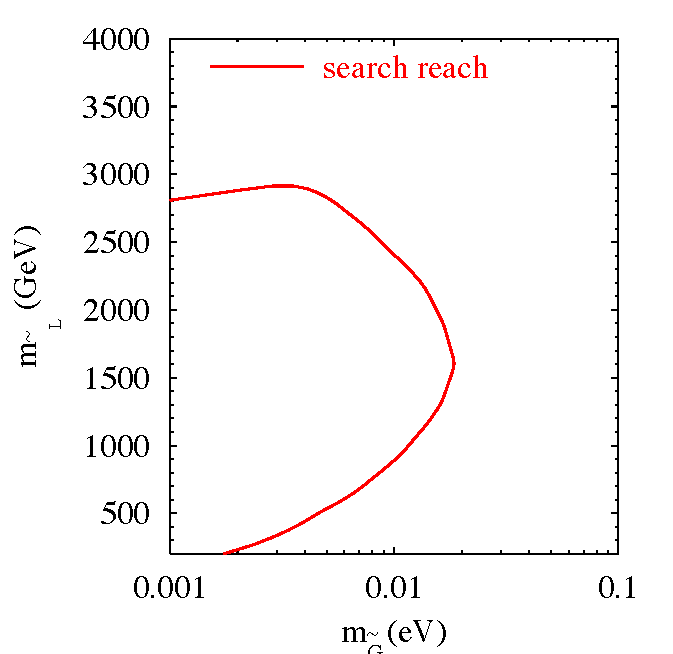
\includegraphics[width=5cm]{Fig1.pdf}
    \caption{...caption...}
    \label{fig:projname:plot1}
  \end{center}
\end{figure}
%% ~\newline~
%% To reference the main parts of the documents, use standard latex commands, with a prefix sec: and cha:.
%%
%% Examples: cha:nnlo will point to Chapter~\ref{cha:nnlo}.
%% Most likely, the conveners will fix these references at the end.
\end{itemize}
~\newline~
To use macros, define them locally, but then un-define them at the end of your local tex file.

Examples `` \Herwig{} `` is written using a macro, which is defined
in the local tex file, and undefined at the end of it.

\subsection{you can write subsections...}
Example of citation: in Ref.~\cite{Belanger:2014vza}

\subsubsection{and subsubsections...}

%= undefine macros (MANDATORY) ====================
\let\Herwig\undefined
\let\Pythia\undefined
\let\Sherpa\undefined
\let\Rivet\undefined
\let\Professor\undefined
\let\eps\undefined
\let\mc\undefined
\let\mr\undefined
\let\mb\undefined
\let\tm\undefined




